\chapter{Solución desarrollada}

\lettrine{E}{n} este capítulo mostraremos una serie de capturas de la solución desarrollada, centrándonos en la parte que se refiere a la resolución de los casos de uso expuestos en \ref{chap:cu}.

\section{Sección de comentarios}

\begin{figure}[H]
	\centering
	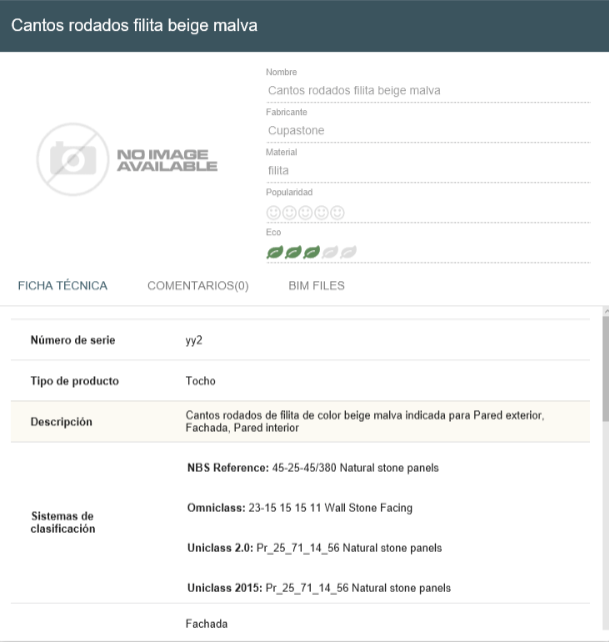
\includegraphics[width=0.5\textwidth]{imaxes/sectComment.png}
	\label{seccom}
	\caption{Sección de comentarios en la ficha de articulo.}
\end{figure}


\section{Publicación de comentarios}

\begin{figure}[H]
	\centering
	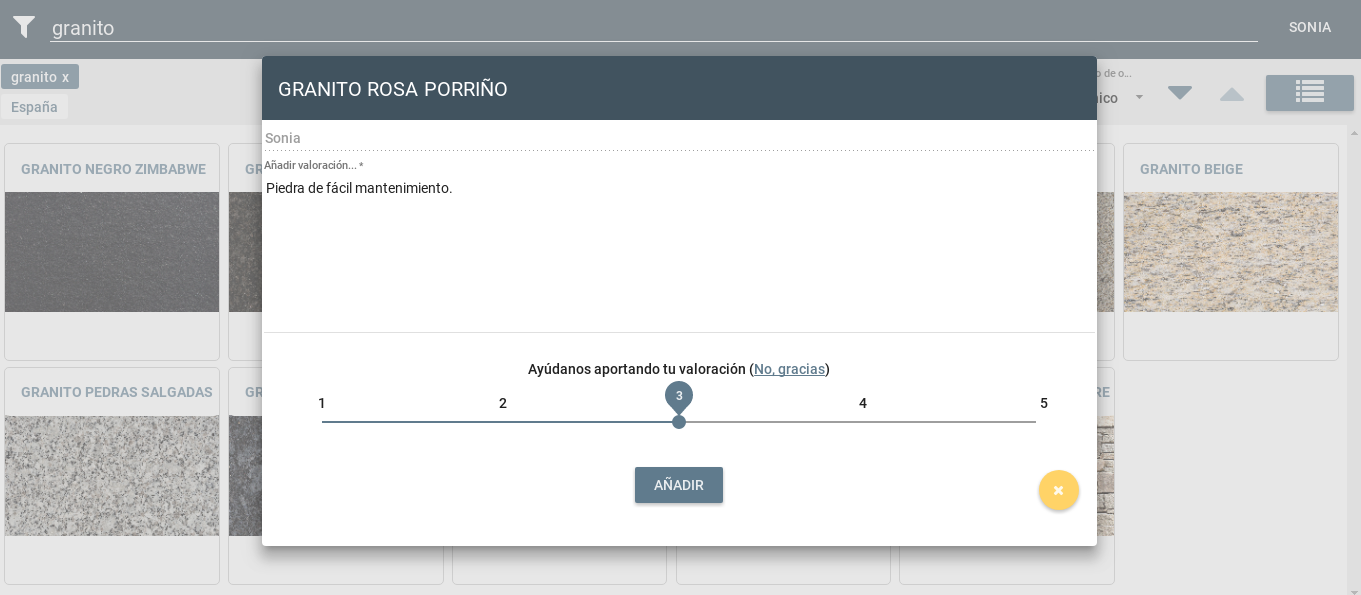
\includegraphics[width=0.75\textwidth]{imaxes/publicComment.png}
	\label{pubcom}
	\caption{Publicación de comentarios.}
\end{figure}

\section{Edición y eliminación de comentarios}

\begin{figure}[H]
	\centering
	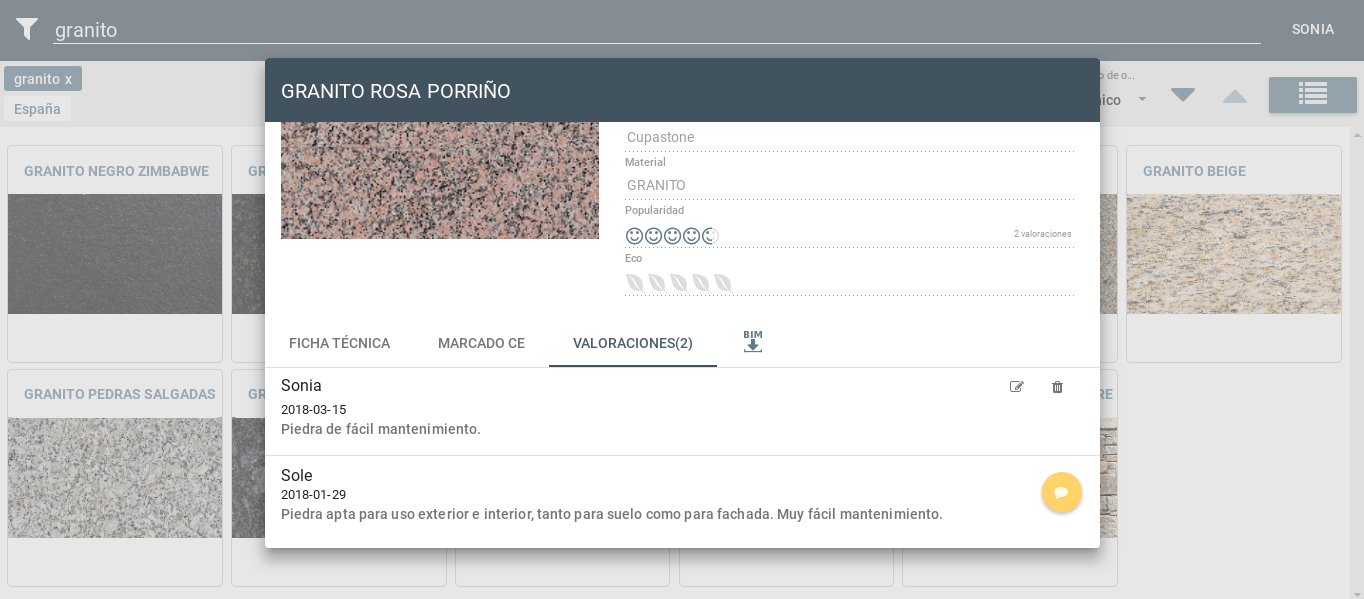
\includegraphics[width=0.75\textwidth]{imaxes/editComment.png}
	\label{edcom}
	\caption{Edición y eliminación de comentarios.}
\end{figure}

\paragraph{Trabajo futuro}

En el apartado de contenido extra se incluyen una serie de capturas que documentan una propuesta de rediseño y modernización de la interfaz.